\titre{Ressources :} Cormen-Leiserson-Rivest-Stein : Algorithmique (Partie Algorithmes pour les graphes) \\
www.sagemath.org \\

\titre{Graphe :} Un graphe $G$ est un couple $(S,A)$ où $S$ est un ensemble fini (les sommets) et $A \subset S\times S$ (les arêtes) \\
Dans un graphe non orienté, les couples $(a,b)$ et $(b,a)$ désignent la même arête. \\
Dans un graphe orienté les arcs $(a,b)$ et $(b,a)$ sont distincts. On dit que l'arc $(a,b)$ part du sommet $a$ et arrive au sommet $b$.\\

\titre{Exemple :} $G = (S,A)$ non orienté avec $S = \{1,2,3,4\}$ et $A=\{(1,2),(1,3),(2,4),(3,4)\}$\\
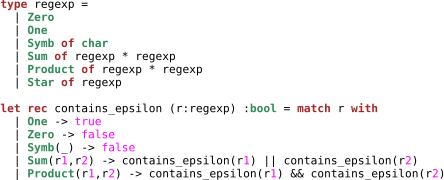
\includegraphics[width=50px]{Images/fig1.pdf}\\

\titre{Exemple :} $G'=(S',A')$ un graphe orienté avec $S'=\{(1,2),(1,3),(2,4),(3,4),(4,2),(1,1)$\\
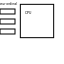
\includegraphics[width=50px]{Images/fig2.pdf}\\

\titre{Adjacence :} Soit $(u,v)$ une arête de $G$. On dit que $v$ est adjacent à $u$\\
\titre{Rq :} Si $G$ est non orienté alors l'adjacence est symétrique.\\

\titre{Degré :} Le degré sortant d'un sommet $u$ de $G$ est le nombre de sommets de $G$ adjacents à $u$. \\
Le degré entrant d'un sommet $v$ de $G$ est le nombre de sommets de $G$ auxquels $v$ est adjacent. \\
Pour un graphe orienté, on appelle degré la somme du degré sortant et du degré entrant. \\
Pour un graphe non orienté, dégré sortant = degré entrant et on note simplement degré. C'est le nombre d'arêtes \titre{incidentes} au sommet.\\

\titre{Exemple :}\\
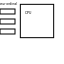
\includegraphics[width=50px]{Images/fig2.pdf}
$D_s(2) = 3 D_e(2) = 2 D(2) = 5$ \\

\titre{Lemme des poignées de main :} Soit $G = (S,A)$ un graphe. Alors $\displaystyle{\sum_{s\in S}D(s) = 2|A|}$\\

\titre{Application :} Si il y a 7 équipes il est impossible de faire que chacune joue contre 5 autres équipes (car alors $2|A| = 35$). \\

\titre{Propriété :} Dans un graphe non orienté, il y a toujours au moins deux sommets avec le même degré.\\

\titre{Preuve :} Soit $n$ le nombre de sommets de $G$. Les degrés possibles sont $\{0, \ldots, n-1\}$. Il ne peut pas y avoir à la fois un sommet de degré $0$ et un sommet de degré $n-1$, donc il y a en réalité $n-1$ degrés possibles, pour $n$ sommets, donc il y a obligatoirement une répétition. \\

\titre{Conséquence :} Dans une soirée il y a toujours au moins 2 personnes qui ont le même nombre d'amis présents. \\

\titre{Egalité et isomorphie :} Deux graphes $G = (S,A)$ et $G' = (S',A')$ sont égaux si $S = S'$ et $A = A'$. \\
Deux graphes $G=(S,A)$ et $G'=(S',A')$ sont isomorphes si il existe une bijection $f$ de $S$ dans $S'$ (appelé ré-étiquetage de $S$ en $S'$) telle que $(a,b) \in A \equi (f(a),f(b)) \in A'$. \\

\titre{Exemple} : $S = \{1,2,3,4\} A = \{(1,2),(1,3),(2,4),(3,4)\}$ et $S'=\{a,b,c,d\} A'=\{(b,c),(c,d),(b,a),(d,a)\}$ sont isomorphes par $$f\ffonc{a}{1}$$ $$f\ffonc{b}{2}$$ $$f\ffonc{c}{4}$$ $$f\ffonc{d}{3}$$
